\documentclass[11pt]{article}
\usepackage{../cs170}


\def\title{Homework 9}
\def\duedate{11/1/2023, at 10:00 pm (grace period until 11:59pm)}

\begin{document}
\maketitle


Due \textbf{\duedate}

\question{Study Group}
List the names and SIDs of the members in your study group.
If you have no collaborators, you must explicitly write ``none''.

\begin{solution}
	None in particular, I got some help on problem 5 and problem 4c during homework parties and office hours but
	besides that the remainder of the work is entirely my own.
\end{solution}

\newpage

\question{Canonical Form LP}
Recall that any linear program can be reduced to a more constrained \emph{canonical form} where all variables are non--negative, the constraints are given by $\leq$ inequalities, and the objective is the maximization of a cost function. 

\noindent More formally, our variables are $x_i$. Our objective is $\max c^\top x = \max \sum_i c_i x_i$ for some constants $c_i$. The $j$th constraint is  $\sum_i a_{ij} x_i \leq b_j$ for some constants $a_{ij}, b_j$. Finally, we also have the constraints $x_i \geq 0$.

\noindent An example canonical form LP: 
\begin{center}
$\mbox{ maximize } 5x_1 + 3x_2$
\begin{align*}
\text{subject to } \begin{cases} x_1 + x_2 - x_3 \leq 1 \\
-(x_1 + x_2 - x_3) \leq -1 \\
-x_1 + 2x_2 + x_4 \leq 0 \\ 
-(-x_1 + 2x_2 + x_4) \leq 5 \\
x_1, x_2, x_3, x_4 \ge 2
\end{cases}
\end{align*}
\end{center} 

\noindent For each of the subparts below, describe how we should modify it to so that it satisfies canonical form. If it is impossible to do so, justify your reasoning. Note that the subparts are independent of one another.
\begin{subparts}
  \subpart Min Objective: $\min \sum_i c_i x_i$

  \begin{solution}
  	We flip the signs of all \(c_i\) and turn the problem into a maximization problem. This satisfies the 
	canonical form, since none of the constraint equations are affected and the objective is now a max.  
  \end{solution}
  \subpart Lower Bound on Variable: $x_1 \geq b_1$

  \begin{solution}
  	Flip the sign on both ends to get \(-x_1 \le -b_1\). This turns the inequality into the proper 
	form with the variables being set less than some value \(b_1\), as desired. 
  \end{solution}
\subpart Bounded Variable: $b_1 \leq x_1 \leq b_2$

\begin{solution}
	Split the inequality into two parts: \(b_1 \le x_1\) and \(x_1 \le  b_2\). The latter inequality is fine 
	since that's already in canonical form, but we flip the first inequality to satisfy the canonical form: 
	\(-x_1 \le  -b_1\). Leaving us with \(x_1 \le  b_2\) and \(-x_1 \le  -b_1\). 
\end{solution}
  \subpart Equality Constraint: $x_2 = b_2$

  \begin{solution}
  	Split this equality into \(x_2 \ge  b_2\) and \(x_2 \le  b_2\), whose solution is that \(x_2 = b_2\). Then, 
	flip the first inequlaity to \(-x_2 \le  -b_2\), leaving us with \(x_2 \le  b_2\) and \(-x_2 \le  -b_2\). 
  \end{solution}
  \subpart More Equality Constraint: $x_1 + x_2 + x_3 = b_3$

  \begin{solution}
	  Nothing changes here compared to the previous part, this is just an equality with more variables 
	  attached to it, so we do the same thing: split the inequality up giving us: \(x_1 + x_2 + x_3 \le  b_3\)
	  and \(-x_1 - x_2 - x_3 \le  -b_3\). 
  \end{solution}
    \subpart Absolute Value Constraint: $|x_1+x_2| \leq b_2$

	\begin{solution}
		We can get rid of the absolute value by turning this equation into \(x_1 + x_2 \le  b_2\) and 
		\(x_1 + x_2 \ge  -b_2\), and the latter equation can be rewritten as \(-x_1 - x_2 \le  b_2\). This 
		leaves us with:
		\begin{align*}
			x_1 + x_2 &\le  b_2\\
			-x_1 - x_2 &\le  b_2
		\end{align*}
		Then, since \(x_1, x_2 \) are both real varaibles, we can use part (i) to write them 
		in terms of new dummy variables that are constrained to be positive: let \(x_1 = a -b\) and 
		\(x_2 = c - d\) where \(a, b, c, d \ge  0\). From these two equalities, we have the constraints:
		\begin{align*}
			a - b - x_1 &\le 0\\
			-a + b + x_1 & \le 0\\
			c - d - x_2 &\le 0\\
			-c + d + d_2 &\le 0
		\end{align*}
		Then, we have the two inequalities from the original absolute value on top of this:
		\begin{align*}
			a - b + c - d & \le b_2\\
			-a + b - c + d& \le  b_2
		\end{align*}
	\end{solution}
    \subpart Another Absolute Value Constraint: $|x_1 + x_2| \geq b_2$

	\begin{solution}
		This follows the same approach as the previous problem: first we split the inequality into 
		\(x_1 + x_2 \ge  b_2\) and \(x_1 + x_2 \le -b_2\), and the first equation we rewrite as 
		\(-(x_1 + x_2) \le  -b_2\). I imagine the difficulty in this problem (and the reason 
		it became optional) comes from actually invoking 
		part (i) and writing the full inequality out. 
	\end{solution}
  \subpart Min Max Objective: $\min \max (x_1,x_2)$

  \emph{Hint: use a dummy variable!}

  \begin{solution}
  	Rephrase the objective as \(\max \min (-x_1, -x_2)\), and let \(\min(-x_1, -x_2)\) be the objective 
	equation. Then, we need to find a way to express \(\min(-x_1, -x_2)\) in terms of a linear equation.  
  \end{solution}


  \subpart Unbounded Variable: $x_4 \in \R$

  \emph{Hint: how can you represent any real number as an operation on two positive numbers?}

  \begin{solution}
  	Introduce new variables \(a, b \ge  0\), and express \(x_4 = a - b\), so this would come out to the 
	inequalities:
	\begin{align*}
		x_4 &\le  a - b\\
		x_4 &\ge  a - b
	\end{align*}
	which we can then convert into:
	\begin{align*}
		a - b - x_4 &\le  0\\
		-a + b + x_4 & \le 0
	\end{align*}
  \end{solution}
\end{subparts}

\newpage

\question{Baker}


You are a baker who sells batches of brownies and cookies (unfortunately no brookies... for now). Each brownie batch takes 4 kilograms of chocolate and 2 eggs to make; each cookie batch takes 1 kilogram of chocolate and 3 eggs to make. You have 80 kilograms of chocolate and 90 eggs. You make a profit of 60 dollars per brownie batch you sell and 30 dollars per cookie batch you sell, and want to figure out how many batches of brownies and cookies to produce to maximize your profits.

\begin{subparts}
\subpart Formulate this problem as a linear programming problem; in other words, write a linear program (in canonical form) whose solution gives you the answer to this problem. Draw the feasible region, and
find the solution using Simplex. 

\begin{solution}
	A similar problem was done in lecture: we'll use \(x_1\) to represent the number of brownies and \(x_2\) be 
	the number of cookies. Therefore, we'd like to maximize the equation \(60x_1 + 30x_2\), subject
	to the constraints:
	\begin{align*}
		4x_1 + x_2 \le 80\\
		2x_1 + 3x_2 \le  90	
	\end{align*}
	along with \(x_1, x_2 \ge  0\). This can be converted into the equations:
	\begin{align*}
		x_2 \le  80 - 4x_1\\
		x_2 \le 90 - 2x_1
	\end{align*}
	From here, we can plot \(x_2\) and \(x_1\) on a graph, which looks like this:
	\begin{center}
		\begin{tikzpicture}[yscale=0.04, xscale=0.08]
			\draw (-10, 0) -- (100, 0) node[right] {$x_1$};
			\draw (0, -10) -- (0, 100) node[above] {$x_2$};
			\draw[domain=-5:25, color = red] plot (\x, {80 - 4*\x}) node[right] {$x_2 = 80 - x_1$};
			\draw[domain = -5:60, color = orange] plot (\x, {30 - 2/3 * \x}) node[right] 
				{$x_2 = 30 -\frac{2}{3}x_1$};
			\filldraw[pattern=north east lines] (0, 0) -- (0, 30) -- (15, 20) -- (20, 0) -- cycle;
		\end{tikzpicture}
	\end{center}
	The hatched region defines the region where all constraints are satisfied. The extrema, computed
	using Desmos, are (0, 0), (0, 30), (15, 20) and (20, 0). Using Simplex, it runs like this:
	\begin{itemize}
		\item Start at (0, 0), look at adjacent vertices: (0, 30) and (20, 0)
		\item (0, 30) has an objective value of 900, and (20, 0) has an objective value of 1200, so we 
			move to (20, 0) since (0,0) has an objective value of 0. 
		\item From (20, 0), neighbouring vertices are (0, 0) and (15, 20), and since (15, 20) has an objective
			value of \(1500 \ge  1200\) then we move to (15, 20).
		\item Neighbouring vertices from (15, 20) are (20, 0) and (0, 30), both of which have objective 
			values lower than (15, 20), so we return (15, 20) as the maximum point. 
	\end{itemize}
\end{solution}
\subpart Suppose instead that the profit per brownie batch is $C$ dollars and the profit per cookie batch remains at 30 dollars. For each vertex you listed in the previous part, give the range of $C$ values for which that vertex is the optimal solution.

\begin{solution}
	Firstly, notice that (0,0) will never be an optimal point, since we can always make cookies. 
	Therefore, there are only three vertices that we 
	really need to check: (20, 0), (15, 20) and (0, 30). I'll go in that order. 
	
	(20, 0) has an objective value of \(20C\), and this is optimal when \(20C > 900\) and \(20C > 15C + 600\).
	The first equation gives  \(C > 45\) and the second gives \(5C > 600 \implies C > 120\), so 
	\(C > 120\) makes (20, 0) the optimal solution. 

	(15, 20) has an objective value of \(15C + 600\), and this is optimal when \(15C + 600 > 900\) and 
	\(15 C + 600 > 20C\). The first equation gives \(C > 20\), and the second gives \(C < 120\). Therefore, 
	this point is optimal when \(20 < C < 120\). 
	
	Then, this leaves (0, 30) to be optimal when \(C < 20\). 
\end{solution}
\end{subparts}

\newpage

\question{Meal Replacement}

Jonny is planning an ``Introduction to CS Theory" overnight summer camp for penguins in Antarctica. Penguins can't solve problems well when they're hungry, so Jonny wants to secure an emergency source of food in case polar bears sneak in and eat everything in the igloo. Unfortunately, he is on a tight budget, and in order to accommodate as many penguins as possible, he needs to minimize the cost of food while still meeting the penguins' minimum dietary needs.

\noindent Every penguin needs to consume at least 600 calories of protein per day, 800 calories of carbs per day, and 500 calories of fat per day. Jonny has three options for food he's considering buying: salmon, bread, and squid. The composition of each food is provided in the following table:

\begin{center}
    \begin{tabular}{|m{6em}|m{5em}|m{8.4em}|m{7em}|m{6.2em}|}
        \hline
         \textbf{Food Type} & \textbf{Price per Pound} & \textbf{Protein Calories per Pound} & \textbf{Carb Calories per Pound} & \textbf{Fat Calories per Pound} \\
         \hline
         Salmon & 6 & 400 & 0 & 150\\
         \hline
         Bread & 1 & 50 & 300 & 25\\
         \hline
         Squid & 8 & 300 & 100 & 200\\
         \hline
    \end{tabular}
\end{center}

\noindent Our goal is to find a combination of these options that meets the penguins' daily dietary needs while being as cheap as possible.

\begin{subparts}
\subpart Formulate this problem as a linear program. 

\begin{solution}
	Let \(x_1\) be the amount of salmon, \(x_2\) be the amount of bread, and \(x_3\) be the amount of squid. 
	Then, the problem wants us to minimize \(6x_1 + x_2 + 8x_3\), subject to the constraints:
	\begin{align*}
		400x_1 + 50x_2 + 300x_3 &\ge  600\\
		300x_2 + 100x_3 &\ge 800\\
		150x_1 + 25x_2 + 200x_3 &\ge 500
	\end{align*}
	So that this is in canonical form, we can rephrase this as maximizing \(-6x_1 - x_2 - 8x_3\) 
	subject to 
	\begin{align*}
		-400x_1 - 50x_2 - 300x_3 &\le -600\\
		-300x_2 - 100 x_3 &\le  -800\\
		-150x_1 - 25x_2 - 200x_3 & \le  -500
	\end{align*}
	and \(x_1, x_2, x_3 \ge  0\).
\end{solution}
\subpart Take the dual of your LP from part (a).

\begin{solution}
	Before computing the dual, we first identify \(A, \vec b, \vec c\) :
	\begin{align*}
		A &= -\begin{bmatrix} 400 & 50 & 300\\ 0 & 300 & 100\\150 & 25 & 200\end{bmatrix} \\
		\vec b &= -\begin{bmatrix} 600\\800\\500 \end{bmatrix} \\
		\vec c &= -\begin{bmatrix} 6 \\ 1\\ 8 \end{bmatrix} 
	\end{align*}
	To construct the dual, we minimize \(\vec b^\top y\) subject to the constraints \(A^\top \vec c \ge y\), 
	meaning we have the system:
	\[
		-\begin{bmatrix} 400 & 0 & 150\\50 & 300 & 25\\300 & 100 &200 \end{bmatrix}
		\begin{bmatrix} y_1 \\ y_2 \\ y_3 \end{bmatrix}	\ge  \begin{bmatrix} -6 \\ -1 \\ -8 \end{bmatrix} 
	\] 
	and we want to minimize \(-600y_1 - 800y_2 - 500y_3\). Putting this in canonical form, this means 
	we want to maximize \(600y_1 + 800y_2 + 500y_3\) subject to the constraints:
	\begin{align*}
		400y_1 + 150y_3 \le  6\\
		50 y_1 + 300y_2 + 25y_3 \le 1\\
		300y_1 + 100y_2 + 200y_3 \le  8
	\end{align*}
\end{solution}
\subpart Suppose now there is a pharmacist trying to assign a price to three pills, with the hopes of getting us to buy these pills instead of food. Each pill provides exactly one of protein, carbs, and fat. 
Interpret the dual LP variables, objective, and constraints as an optimization problem from the pharmacist's perspective.

\begin{solution}
	Firstly, the variables \(y_1, y_2, y_3\) can be interpreted as the price per calorie of each nutrient. 
	In this way, we can interpret each constraint as the statement that buying the pharmacist's pills 
	are more worth it than buying the corresponding food type, since this is the only way the pharmacist 
	can convince us to buy their product over the real thing. 

	For instance, the equation 
	\(400y_1 + 150 y_3 \le  6\) constrains the price of \(y_1, y_3\) so that purchasing from the pharmacist 
	is more worth it than buying the salmon, which provides the same amount of calories for each nutrient. Then, 
	the intersection of all three of these constraints corresponds to the region in which buying the pills 
	from the pharmacist to buy the nutrients is always cheaper than buying its corresponding food type.

	In this framework, the objective equation represents the profit that the pharmacist can 
	make, with the coefficients representing 
	how much of each nutrient the penguins need. 
\end{solution}
\end{subparts}

\newpage

\question{Practice With Residual Graphs}

\begin{subparts}
\subpart 
Consider the following network and flow on this network. An edge is labelled with its flow value (in blue) and capacity (in black). e.g. for the edge $(s, a)$, we are currently pushing 2 units of flow on it, and it has capacity 7.
\begin{center}
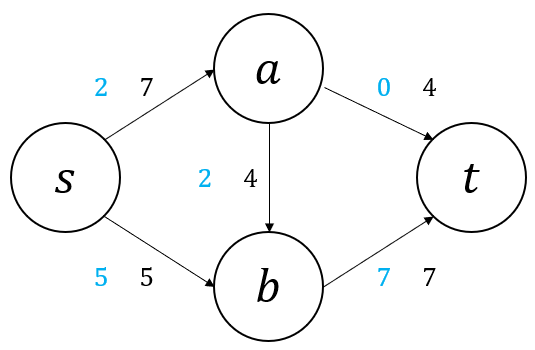
\includegraphics[width=3in]{flow-example.PNG}
\end{center}
Draw the residual graph for this flow.

\begin{solution}
	Based on the description of the residual graph in lecture:
	
	\begin{center}
		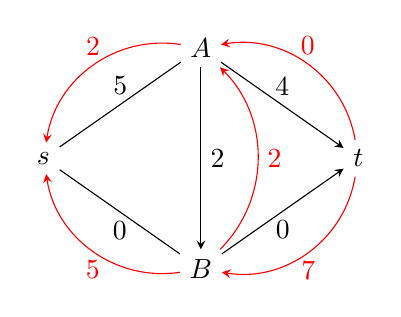
\begin{tikzpicture}[scale=2]
			\node (s) at (0, 0) {$s$};
			\node (a) at (1, 0.7) {$A$};
			\node (b) at (1, -0.7) {$B$};
			\node (t) at (2, 0) {$t$};
			\draw[-stealth] (s) -- node[midway, above] {5} (a) -- node[midway, above] {4} (t);
			\draw [-stealth] (s) -- node[midway, below] {0} (b) -- node[midway, below] {0} (t);
			\draw[-stealth] (a) -- node[midway, right] {2} (b);
			\draw[-stealth, out=-45, in = -135, relative, red] (a)  to node[midway, above] {2} (s) ;
			\draw[-stealth, out = 45, in = 135, relative, red] (b) to node[midway, below] {5} (s);
			\draw[-stealth, out = -45, in = -135, relative, red] (t) to node[midway, above] {0} (a);
			\draw[-stealth, out = 45, in = 135, relative, red] (t) to node[midway, below] {7} (b);
			\draw[-stealth, out = -45, in = -135, relative, red] (b) to node[midway, right] {2} (a);
		\end{tikzpicture}
	\end{center}

\end{solution}

\subpart 
We are given a network $G = (V, E)$ whose edges have integer capacities $c_e$, and a maximum flow $f$ from node $s$ to node $t$. Explicitly, $f$ is given to us in the representation
of integer flows along every edge $e$, $\{f_e\}_{e \in E}$. 

However, we find out that one of the capacity values of $G$ was wrong: for edge $(u, v)$, we used $c_{uv}$ whereas it really should have been $c_{uv} - 1$.
This is unfortunate because the flow $f$ uses that particular edge at full capacity: $f_{uv} = c_{uv}$.
To fix this, we could run Ford Fulkerson from scratch, but there's a faster way.

Describe an algorithm to fix the max-flow for this network in $O(|V|+|E|)$ time. \textbf{Give a three-part solution.}

\begin{solution}

	\textbf{Algorithm Description:} We first find a path from \(t\) to \(s\) on the residual graph
	that has nonzero edge weight, and 
	subtract one from the flow along that path and add 1 to the capacity for every edge excluding \((u, v)\). 
	Then, find another path from \(s \to t\) that avoids 
	edge \((u, v)\), and send 1 flow along that path, if such a path exists. This condition of avoiding 
	\((u, v)\) can be enforced by deleting all edges that have zero weight. 

	\textbf{Proof of Correctness:} To correct the flow, we just have to find a path from \(t \to s\) that uses 
	edge \((u, v)\) and subtract 1 flow along that path, since by subtracting 1 we correct the flow along 
	edge \((u, v)\) to fit the proper capacity. Then, since we've reduced the flow in the graph by 1, we need to 
	find another path this 1 unit of water take from \(s \to t\), so we need to find another path from 
	\(s \to t\). 

	The only instance where this path will not exist is when \((u, v)\) lies on the min cut of the graph, 
	since we've proved in lecture that max flow = min cut. Therefore, if \((u, v)\) lies on the 
	min cut, then the max flow is reduced by 1, so the second part of our algorithm doesn't find 
	another valid path. 

	\textbf{Runtime Analysis:} This algorithm can be implemented quite easily by running DFS twice, once 
	for finding a path from \(t\to s\) and then another time from finding a path from \(s \to t\). Each 
	instance of DFS takes \(O(|V| + |E|)\) time, so the total runtime is \(O(|V| + |E|)\).
\end{solution}
\end{subparts}

\newpage

\question{(Extra Credit) Huffman and LP}

Consider the following Huffman code for characters $a, b, c, d$: $a = 0, b = 10, c = 110, d = 111$. 

Let $f_a, f_b, f_c, f_d$ denote the fraction of characters in a file (only containing these characters) that are $a, b, c, d$ respectively. Write a linear program with variables $f_a, f_b, f_c, f_d$ to solve the following problem: What values of $f_a, f_b, f_c, f_d$ (that can generate this Huffman code) result in the Huffman code using the most bits per character? 

\begin{solution}
	In order to maximize the number of bits per character, we multiply the frequency of each letter 
	by its corresponding bit length, meaning our objetive equation is \(f_a + 2f_b + 3f_c + 3f_d\). 

	Then, recall that the way we generate Huffman codes is based on frequency, meaning that for this particular 
	Huffman code, the character \(a\) must have the highest frequency, then followed by \(b, c \) and \(d\).
	Therefore, one of our constraints is that \(f_d \le  f_c \le  f_b \le  f_a\). Further since the 
	file can only contain these characters, we have the additional constraint tat \(f_a + f_b + f_c + f_d = 1\), 
	which we can formulate into an inequality by writing (utilizing problem 2): 
	\begin{align*}
		f_a + f_b + f_c + f_d &\le  1\\
		-f_a - f_b - f_c - f_d & \le  -1
	\end{align*}
	Then, as for the big constraint of \(f_d \le  f_c \le  f_b \le  f_a\), we can decompose this by enforcing 
	the inequalities pairwise:
	\begin{align*}
		f_d - f_c &\le  0\\
		f_d - f_b &\le  0\\
		f_d - f_a & \le  0\\
		f_c - f_b&\le  0\\
		f_c - f_a &\le  0\\
		f_b - f_a &\le  0
	\end{align*}
	combining these with the earlier two inequalities gives us the full set of inequalities and completes 
	this LP.
\end{solution}
\newpage

\question{(Extra Credit) Flow Decomposition}

Let $G = (V, E)$ be a directed graph, and let $f$ be any $s-t$ flow on this graph. Assume that there is no cycle in the graph where $f_e > 0$ for all edges in the cycle. Design an algorithm to decompose $f$ into the sum of at most $|E|$ path flows. That is, your algorithm should find a set of $s-t$ paths $p_1 \ldots p_k$ and corresponding flow values $F_1 \ldots F_k$ such that:

\begin{itemize}
\item The number of paths $k$ is at most $|E|$
\item $f$ is the sum of $k$ path flows, where the $i$th flow sends $F_i$ units of flow on path $p_i$. That is, for each edge $e$, if $P_e$ is the set of paths in $p_1 \ldots p_k$ that contain $e$, then $\sum_{p_i \in P_e} F_i = f_e$.
\end{itemize}

For example, in the below graph (where each edge $e$ is labelled with $f_e$), one can decompose the flow into $p_1 = ((A, B), (B, C), (C, D)), p_2 = ((A, B), (B, D))$ where $F_1 = 1$, $F_2 = 2$.

\begin{center}
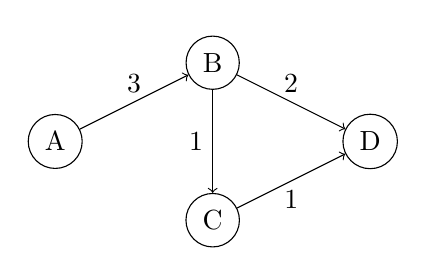
\begin{tikzpicture}
[baseline=(A.base),
 arc/.style={->,thick,>=stealth},
 vertex/.style={draw,circle},]

\node [vertex] at (0cm,0cm) (A) {A};
\node [vertex] at (2cm,1cm) (B) {B};
\node [vertex] at (2cm,-1cm) (C) {C};
\node [vertex] at (4cm,0cm) (D) {D};

\draw (A) + (0cm, .1cm) node [vertex, transparent] (a) {A};
\draw (B) + (0cm, .1cm) node [vertex, transparent] (b) {B};
\draw (C) + (0cm, .1cm) node [vertex, transparent] (c) {C};
\draw (D) + (0cm, .1cm) node [vertex, transparent] (d) {D};

\draw[->] (A) -- node [above] {3} (B);
% \DrawArc AB3
\draw[->] (B) -- node [left] {1} (C);
% \DrawArc BC1
\draw[->] (C) -- node [below] {1} (D);
% \DrawArc CD1
\draw[->] (B) -- node [above] {2} (D);
% \DrawArc BD2
\end{tikzpicture}
\end{center}

Provide the algorithm description and a brief explanation of why your algorithm finds at most $|E|$ paths. 

\emph{Hint: How does Ford-Fulkerson work?}

\newpage

\question{Coding Questions: Max Flow/Min Cut}

For this week’s coding questions, we'll walk through the \textbf{Edmonds Karp} algorithm for max flow and see how to compute the \textbf{Minimum Cut} given a solution to the max flow problem.  There are two ways that you can access the notebook and complete the problems:
\begin{enumerate}
    \item \textbf{On Local Machine}: \texttt{git clone} (or if you already cloned it, \texttt{git pull}) from the coding homework repo, 
    
    \textcolor{blue}{\href{https://github.com/Berkeley-CS170/cs170-fa23-coding}{\texttt{https://github.com/Berkeley-CS170/cs170-fa23-coding}}}
    
    and navigate to the \texttt{hw09} folder. Refer to the \texttt{README.md} for local setup instructions.

    \item \textbf{On Datahub}: Click \textcolor{blue}{\href{https://datahub.berkeley.edu/hub/user-redirect/git-pull?repo=https://github.com/Berkeley-CS170/cs170-fa23-coding}{here}} and navigate to the \texttt{hw09} folder if you prefer to complete this question on Berkeley DataHub.
\end{enumerate}

\noindent Notes:
\begin{itemize}
    \item \textit{Submission Instructions:} Please download your completed submission \texttt{.zip} file and submit it to the Gradescope assignment titled ``Homework 9 Coding Portion''. 
        
    \item \textit{OH/HWP Instructions:} Designated coding course staff will provide conceptual and debugging help during office hours and homework parties.

    \item \textit{Edstem Instructions:} Conceptual questions are always welcome on the public thread. If you need debugging help first try asking on the public threads. To ensure others can help you, make sure to:
        \begin{enumerate}
            \item Describe the steps you've taken to debug the issue prior to posting on Ed.
            \item Describe the specific error you're running into.
            \item Include a few small test cases, alongside both the output you expected to receive and your function's actual output. 
        \end{enumerate}
    If staff tells you to make a private Ed post, make sure to include \textit{all of the above items} plus your full function implementation. If you don't provide them, we will ask you to provide them.
    
    \item \textit{Academic Honesty Guideline:} We realize that code for some of the algorithms we ask you to implement may be readily available online, but we strongly encourage you to not directly copy code from these sources. Instead, try to refer to the resources mentioned in the notebook and come up with code yourself. That being said, we \textbf{do acknowledge} that there may not be many different ways to code up particular algorithms and that your solution may be similar to other solutions available online.
    
\end{itemize}
\end{document}

